% !TEX program = xelatex
\documentclass{exam}
\usepackage{ctex}
\usepackage{fontawesome}
\usepackage{tikz}
\usepackage{epstopdf}
\usepackage{booktabs}
\usepackage{subfigure}
\usetikzlibrary{arrows,decorations.markings}
\usetikzlibrary{decorations.pathreplacing}
\usetikzlibrary{calc}
\qformat{}
\renewcommand{\questionshook}{%
\setlength{\leftmargin}{0pt}%
\setlength{\labelwidth}{-\labelsep}%
}

\begin{document}
  \begin{questions}
    \question 在如下网络中,各主机与各路由器每个端口的IP地址及MAC地址均如图标注:\\
    \begin{figure}[!htb]
      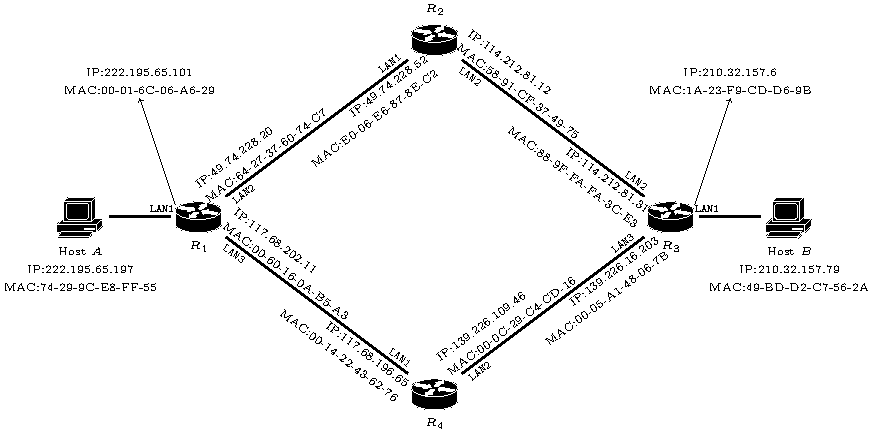
\includegraphics{diag3.pdf}
    \end{figure}
  \\  各路由器的路由表:
    \begin{table}[!htb]
            \centering
      {\footnotesize
      \subtable[$R_1$]
      {\begin{tabular}{c|c|c|c}
      \toprule
     目的IP地址 & 子网掩码 & 下一跳IP & 出口 \\
     \hline
    222.195.65.0 & 255.255.255.0 & 直接相连 & LAN1 \\
    49.74.228.0 & 255.255.0.0 & 直接相连 & LAN2 \\
    117.68.196.0 & 255.255.196.0 & 直接相连 & LAN3 \\
    210.32.128.0 & 255.255.224.0 & 49.74.228.52 & LAN2\\
    210.32.112.0 & 255.255.240.0 & 117.68.196.65 & LAN3\\
    \bottomrule
   \end{tabular}}
   \subtable[$R_2$]
    {\begin{tabular}{c|c|c|c}
      \toprule
     目的IP地址 & 子网掩码 & 下一跳IP & 出口 \\
     \hline
     49.74.228.20 & 255.255.255.0 & 直接相连 & LAN1 \\
     114.212.81.0 & 255.255.255.0 & 直接相连 & LAN2 \\
     222.195.65.0 & 255.255.255.0 & 49.74.228.20 & LAN1 \\
     210.32.157.0 & 255.255.255.0 & 114.212.81.31 & LAN2 \\
     \bottomrule
    \end{tabular}
  }
     \subtable[$R_3$]{
     \begin{tabular}{c|c|c|c}
       \toprule
      目的IP地址 & 子网掩码 & 下一跳IP & 出口 \\
      \hline
      210.32.157.0 & 255.255.255.0 & 直接相连 & LAN1 \\
      114.212.81.0 & 255.255.255.0 & 直接相连 & LAN2 \\
      139.226.0.0 & 255.255.128.0 & 直接相连 & LAN3 \\
      222.195.0.0 & 255.255.64.0 & 114.212.81.12 & LAN2\\
      222.195.64.0 & 255.255.64.0 & 139.226.109.46 & LAN3\\
      \bottomrule
      \end{tabular}
     }
     \subtable[$R_4$]{
     \begin{tabular}{c|c|c|c}
       \toprule
      目的IP地址 & 子网掩码 & 下一跳IP & 出口 \\
      \hline
      117.68.196.0 & 255.255.196.0 & 直接相连 & LAN1 \\
      139.226.0.0 & 255.255.128.0 & 直接相连 & LAN2 \\
      222.195.65.0 & 255.255.255.0 & 117.68.196.65 & LAN1 \\
      210.32.157.0 & 255.255.255.0 & 139.226.16.203 & LAN2 \\
      \bottomrule
      \end{tabular}
     }
     }
    \end{table}
      \\  主机A向主机B发送数据,主机B收到主机A发送过来的数据后将发送消息给A确认,那么分别这两次数据交换中:
    \begin{parts}
    \part 数据途经的路径(要求描述依次经过哪些路由)
    \part 在路径的每条边中的数据单元中的源IP地址、目的IP地址、源MAC地址、目的MAC地址
\end{parts}
\end{questions}
\end{document}
